%!TEX root=../paper.tex

\chapter{Introduction}
\label{sec:intro}

Power efficiency is critical in designing and operating modern microprocessors. In the early 2000s, microprocessor designers have put low power as a first-order concern in designing digital integrated circuits~\cite{pedram2002power, rabaey2009low}, pointing out that the power density of a microprocessor could exceed that of a nuclear reactor should the clock rate continues the conventional Dennard Scaling~\cite{rabaey2002digital}, making heat dissipation a key constraint for estimating total chip power budget. More recently, as the information ecosystem shifts towards the cloud-edge paradigm, power efficiency has been classified as a key design constraint by researchers on both ends. For datacenters, higher hardware power efficiency entails lower total cost of ownership (TCO), which increases the profit margin of an enterprise~\cite{barroso2013datacenter}. For mobile devices, higher efficiency prolongs battery life, which improves user satisfaction~\cite{zhu2017energy}. Therefore, improving microprocessor power efficiency is an important goal for computer architecture researchers today.

While there is significant motivation to improve microprocessor power efficiency, the end of Dennard scaling and Moore's law~\cite{esmaeilzadeh2011dark,theis2017end} have made our design arsenal increasingly limited to achieve this goal. Specifically, it has become increasingly difficult to continue pushing more active cores onto the silicon real estate and relying on parallelism for improving performance while keeping power under control, as is the common practice in the past 10 years, leaving aside the difficulty of programming parallel software. As techniques are being exhausted to optimize conventional general purpose hardware, many researchers have turned to application-specific proposals, notably customized hardware design (i.e. accelerators) to reduce the power wastage of data movement and instruction decoding in general purpose chips~\cite{qadeer2015convolution}. While this approach has proven to be successful in key emerging applications domains, e.g., machine learning~\cite{chen2014diannao, jouppi2017datacenter, caulfield2016cloud, dean2018new}, its design, verification, and manufacturing costs is, however, non-negligible in the fast development cycle of today's technology world. As a result, alternative proposals with lower overhead, wider applicability, and practical power efficiency gains are still highly desirable for chip vendors as well as consumers.

In this thesis, we seek to improve microprocessor power efficiency by optimizing pipeline's timing margin, a long-neglected, but possibly one of the last opportunities where processor efficiency can yet be improved. The significance of this thesis topic is based upon three findings. First, over 10\% power or performance gain can be achieved simply by squeezing down modern microprocessor's existing timing margin, based on real hardware measurement on production CPUs and GPUs~\cite{reddi2010voltage, leng2015safe}, which proves practical benefit can be realized by working on the excess timing margin. Second, timing margin exists for all processor architectures, from CPUs~\cite{reddi2009voltage,reddi2010voltage} to GPUs~\cite{leng2014gpuvolt, leng2015gpu, leng2015safe}, and inevitably in the upcoming accelerators. This is because all pipelined architectures need to prevent from timing failure, caused by chip environment changes, such as unusual temperature, voltage noise, or process corners. Thus, some amount of margin is always required, indicating the opportunity from timing margin is pervasive. Third, to date there is no comprehensive thesis that systematically studies a practical solution that can effectively reduce timing margin in production processors, and hence the implication for the whole computing system layers are yet to be discovered.

Specifically, our thesis focuses on studying the system-level implication of one technique previously proposed to reduce timing margin, i.e. \textit{Active Timing Margin}. The efficiency improvement opportunity from timing margin is like a free meal for processor designers. However, all proposals but active timing margin has not seen wide-adopted success in practicality, including those in the architecture layer~\cite{grochowski2002microarchitectural,ernst2003razor,powell2003pipeline,gupta2008decor,gupta2009event, reddi2009voltage} and system software layer~\cite{reddi2010voltage,miller2012vrsync,leng2015safe, papadimitriou2017harnessing}, either because of the high hardware design overhead, or incompleteness of guaranteeing execution correctness. Active timing margin, on the other hand, uses a hardware loop to adjust chip supply voltage and frequency based on real-time monitored load environment. It incurs low hardware design overhead, and has been tested rigorously on various production processors to pass load environment corner cases~\cite{lefurgy2011active,bowman201222nm,tokunaga20145,grenat20145,bowman20158,webel2015robust,vezyrtzis2018droop,fischer200590nm}. Thus, understanding how active timing margin behaves and saves timing margin in the field, and trying to maximize its efficiency gain with appropriate management has practical impact for designing future computing systems.

\paragraph{Thesis Statement} To maximize the power efficiency gain extracted from reducing timing margin, we must not take the default active timing margin equipped in a microprocessor as it is. Instead, we must include synergistic management across circuit, architecture, and application to aid active timing margin's runtime behavior. Following this tenet, my thesis proposes active timing margin management across temperature, voltage, and process variation, the combination of which deals with all major sources of microprocessor timing margin consumption to maximize the efficiency improvement.

The rest of this chapter is organized as follows. \Sec{sec:intro:work} provides an overview of my research contributions. \Sec{sec:intro:impact} discusses the long-term practical impact of my thesis. \Sec{sec:intro:outline} outlines the rest of the dissertation and \Sec{sec:intro:prev} lists previously published materials that this dissertation draws upon.

\section{Research Contributions}
\label{sec:intro:work}

My Ph.D. research's objective is to study and optimize the next-generation control system that minimizes processor timing margin - a hardware/software collaborative system that works in synergy to dynamically and safely provision timing margin when it is needed, and to maximize the power efficiency gain promised by such active mechanism. Because processor timing margin is designed to combat against a wide variety of parasitic effects such as voltage noise, temperature heating, process variation, and aging. The design and management of an active timing margin system necessitates a solid understanding of all major effects that affect load environments. To judiciously decide where in the system stack should each of these effect be coped with, and how to cope with each of these effects, active timing margin must be established upon the knowledge of the spatial-temporal characteristics of each effect, as well as the causes and consequences of each effect. Following this principle, my Ph.D. research employs a rigorous methodology of experimenting, observing, inducting, and finally optimizing. 

My Ph.D. research dissects timing margin into three major components that it protects against: temperature, voltage, and process variation. These three effects are the main contributors of microprocessor circuit's timing uncertainty. I take a holistic view across system stack, spanning circuit, architecture, and application to decide for each effect what the appropriate active mechanism is while system overhead is minimal. My preliminary work~\cite{leng2015gpu,zu2015adaptive,zu2016tistate} has demonstrated that this approach of matching an effect to a system layer works well to provision timing margin dynamically and improves power efficiency.

For temperature variation, conventional timing margin assumes a worst-case high temperature scenario to allocate timing margin in a microprocessor, while runtime temperature change and the resulting circuit speed variation are neglected. We find that as technology scales down the circuit speed variation at different temperature promises significant timing margin utilization changes, which promises an opportunity to dynamically adjust timing margin based on real time chip temperature. Because chip temperature changes relatively slow (i.e., at millisecond level), we put active timing margin for temperature variation in the firmware/system software. Specifically, we exploit CMOS transistor's \textit{temperature inversion} effect which speeds up circuit under higher temperature. We build \tistates, a temperature-voltage table that is indexed at runtime to set timing margin by setting voltage. The dynamically adjusted voltage improves power efficiency compared to a conventional fixed margin scenario.

For voltage variation, conventional timing margin targets a worst-case scenario where excess $di/dt$ effects causes large voltage droops that slow down circuit significantly. Because these extreme $di/dt$ effects happen very fast (i.e., for tens of cycles), active timing management for voltage variation necessitate fast control loop which needs to be implemented in the hardware. Our study on a commercial POWER7+ processor shows $di/dt$ effects can be dealt with very effectively in this manner, yet the benefit of active timing for $di/dt$ effects strongly depends upon workload characteristics and chip-wide multicore activity. The underlying reason is a result of the interactions between the application characteristics, architecture and the underlying voltage regulator module's loadline effect and IR drop effects. To maximize active timing margin's gains, we introduce workload mapping support to balance compute loads on different active timing margin ``domains''. Appropriate scheduling can double the original power efficiency improvement achieved by active timing margin.

In the spirit of measuring the behavior of each of these environmental effects rigorously and seeking solutions across system stack accordingly, I propose the following research items. \Fig{fig:framework} gives an overview of the proposed cross-layer research.

\begin{sidewaysfigure}
  \centering
  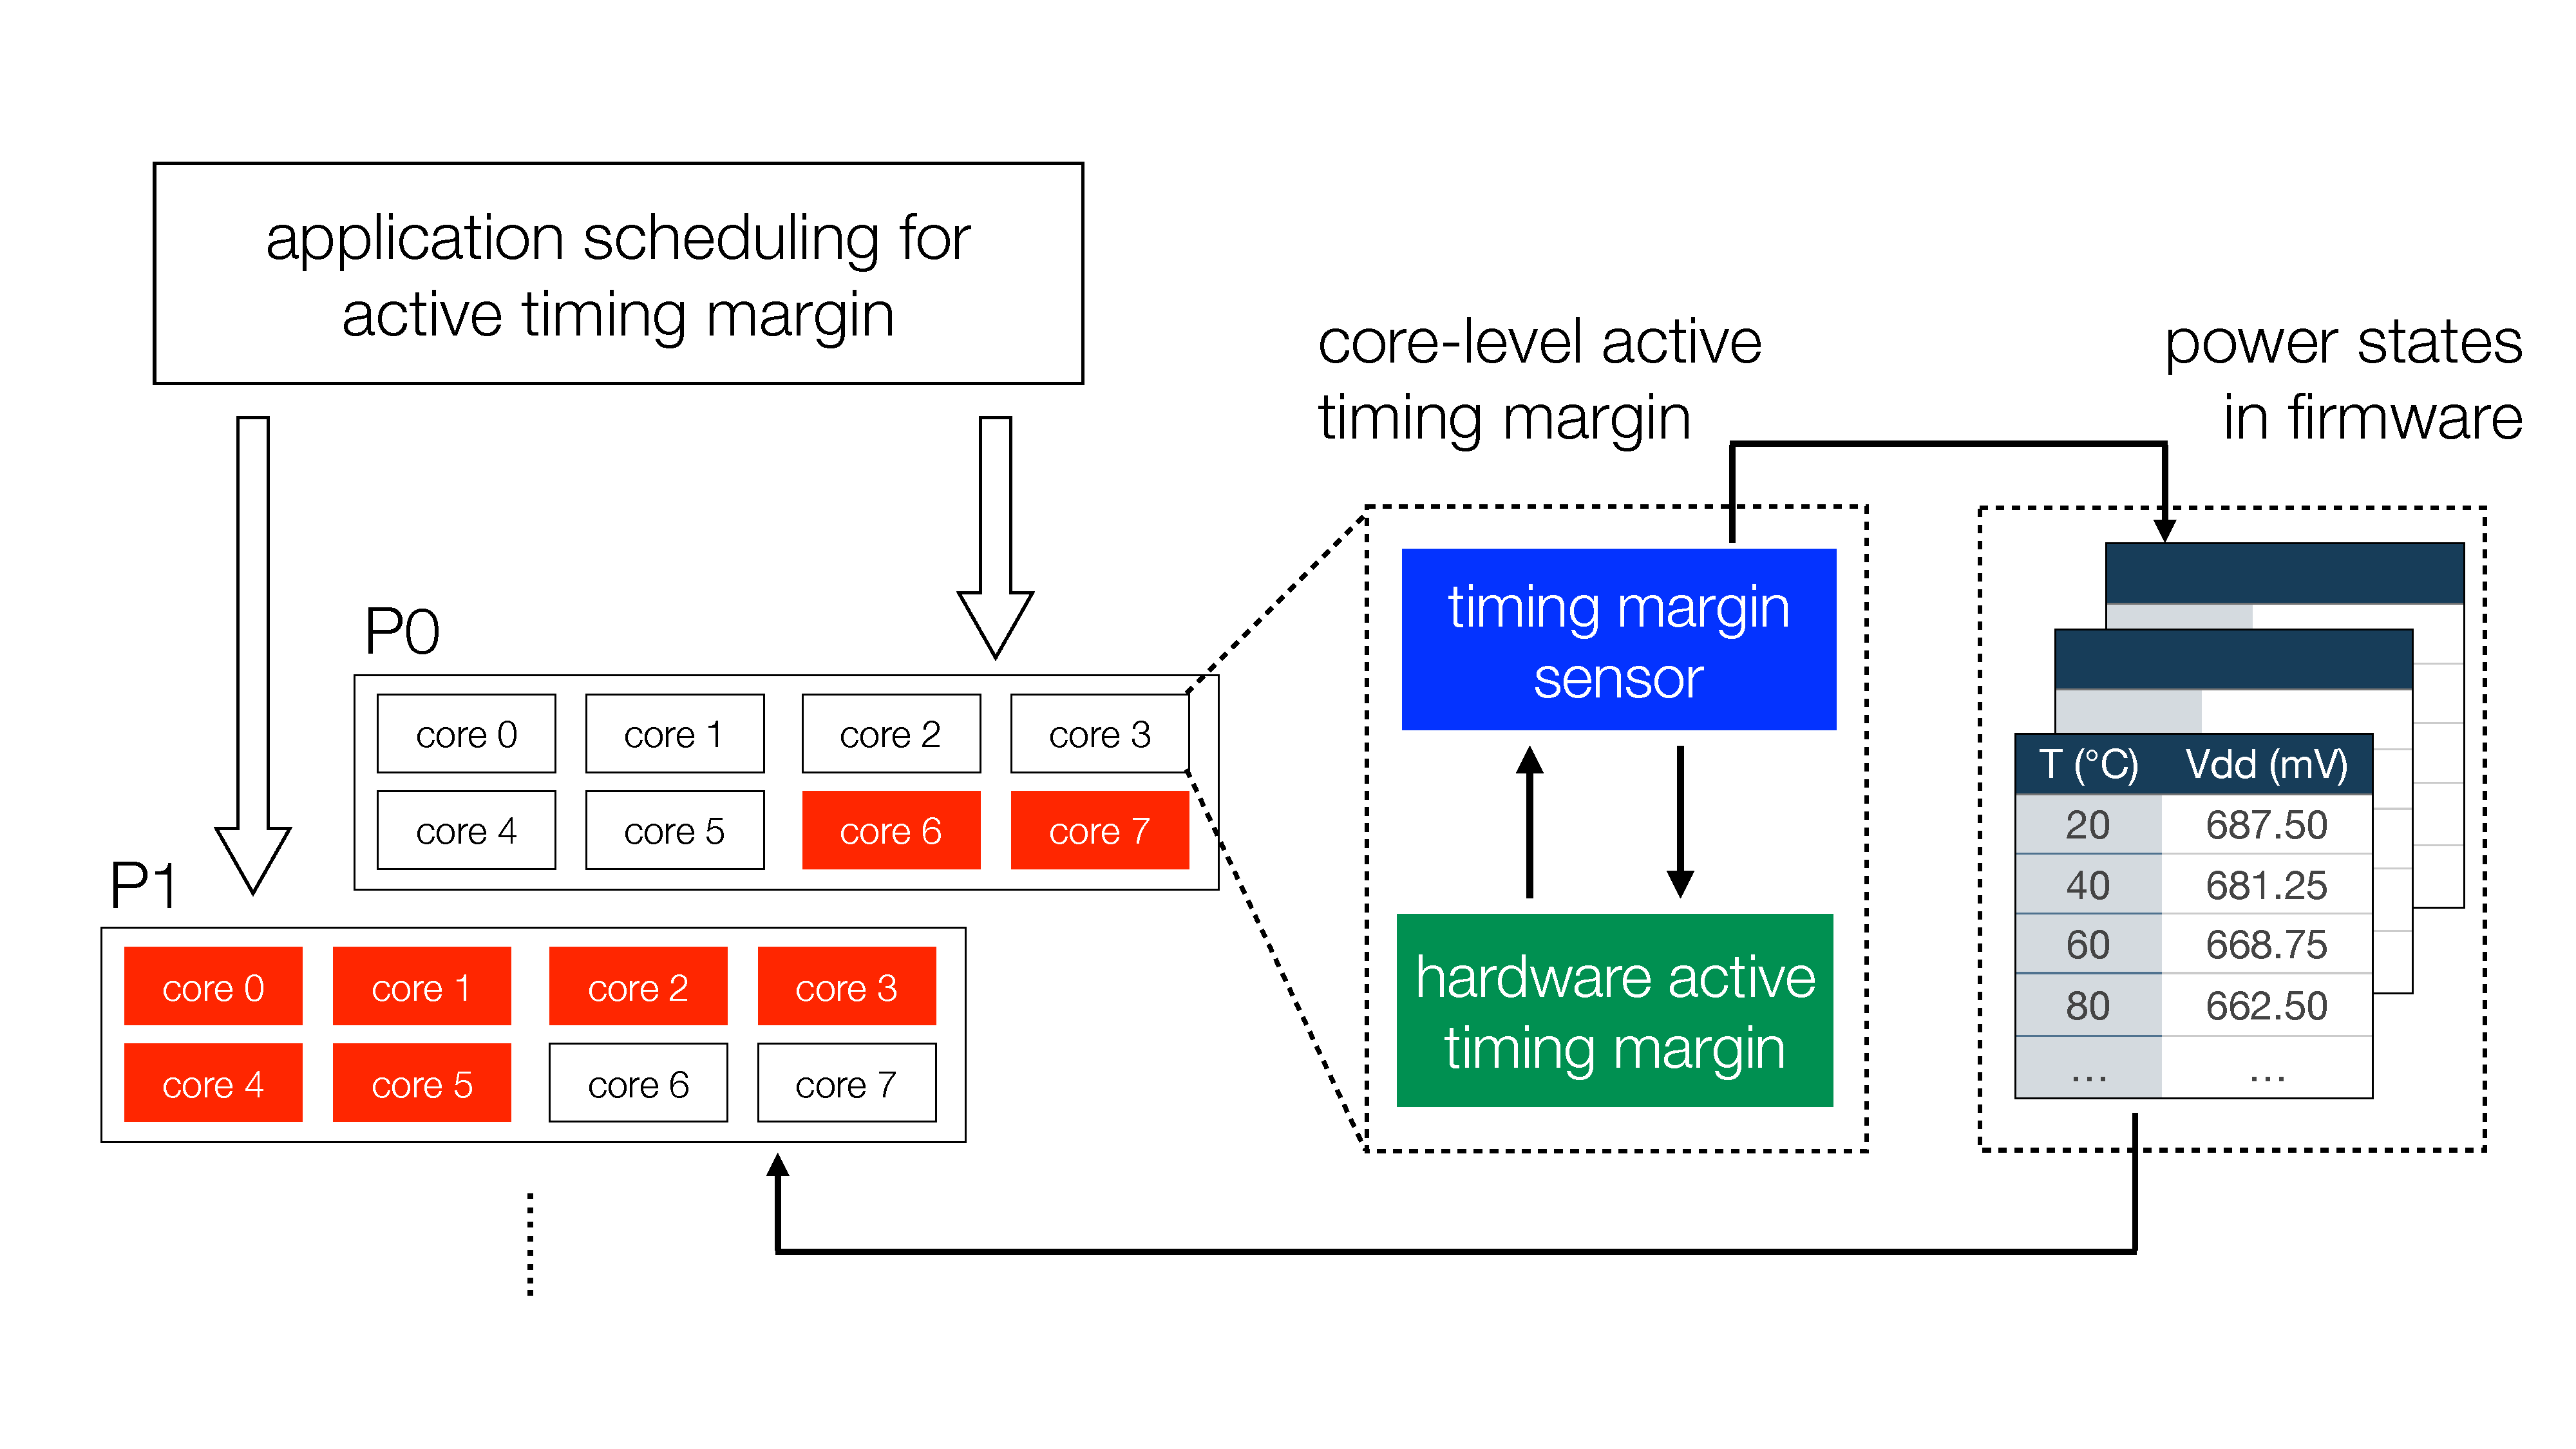
\includegraphics[trim=0 0 0 0, clip, width=\columnwidth]{graphs/intro/sys-overview.pdf}
  \caption{Overview of this thesis's cross-layer research on active timing margin management. We characterizes state-of-the art hardware active timing margin mechanisms such as those that deal with fast $di/dt$ effects, proposes software scheduling techniques to aid aid these active timing chips, and draft firmware power management states to augment existing active timing margin techniques.}
  \label{fig:framework}
\end{sidewaysfigure}

\begin{itemize}
\item \textbf{Firmware Power Management States:} I propose \tistate, a set of power management states that adjust timing margin for different temperature. \tistates target the timing margin opportunity from microprocessor temperature variation, specifically the \textit{temperature inversion} phenomenon in latest CMOS technologies. \tistate is an evolution of classic power management states like P-states. Its table lookup mechanism is succinct and easy to deploy in practice.

\item \textbf{Application Scheduling for Active Margin:} I propose \ams, active margin scheduling that schedules application on a multiple sockets and cores with the awareness of the underlying active timing margin mechanism for $di/dt$ effects. \ams is proposed based on a comprehensive understanding of the effectiveness as well as limitations of hardware active timing margin mechanism that protects against voltage variation. The scheduling solution not only maximize the gains of active timing margin by itself, but also sheds light on how processor power de
\end{itemize}

\section{Long-term Impact}
\label{sec:intro:impact}

The \textit{long-term impact} of my proposal lies in the fact that semiconductor chip forms the fundamental infrastructure for all information technologies, and any improvement to processor power efficiency without changes to abstractions interfacing other system components have the potential of seamlessly benefiting virtually all applications and systems. Active timing margin is one such technique that can be applied to CPUs, GPUs, accelerators. Furthermore, the work presented in this proposal is based on comprehensive measurement on real state-of-the-art hardware, which makes its insights and results a good reference for designers and researchers in this field.

The rest of the proposal is organized as follows. \Sec{sec:motivation} explains the inefficiency of the timing margin in today's processor, and motivates the need for designing active timing margin, as well as the need to maximize active timing margin's power saving potential. \Sec{sec:tistate} and \Sec{sec:ags}describe the proposed \tistates and \ams respectively. \Sec{sec:conc} provides a retrospective and prospective view of the proposed work. The retrospective part summarizes the principles distilled from the work so far about building and optimizing for an active timing margin system; the prospective part suggests next steps and outlines specific research items planned in preparing the final dissertation.rocessor (micro-)architecture or application features.

\section{Dissertation Organization}
\label{sec:intro:outline}

The rest of my dissertation is organized as follows. \Sec{sec:background} introduces the preliminary knowledge of Web computing. \Sec{sec:motivation} quantitatively demonstrates the need for high-performance and energy-efficient computation in the mobile Web, which directly motivates the research theme of my work. \Sec{sec:arch}, \Sec{sec:runtime}, and \Sec{sec:lang} describe the proposed \webcore, \webrt, and \greenweb at the architecture, runtime, and programming language layer, respectively. \Sec{sec:conc} provides a retrospective and prospective view of my dissertation work. The retrospective part summarizes the principles distilled from this work on building a high-performance while energy-efficient mobile Web computing system; the prospective part suggests next steps for generalizing the principles and outlines potential research items for future work.

\section{Previously Published Material}
\label{sec:intro:prev}

This dissertation contains materials that are previously published in peer-reviewed conferences and journals:

\textbf{\Sec{sec:background}}. The network-versus-computer analysis in \Sec{sec:motivation:perf} contains results from the following paper: \textit{The Role of the CPU in Energy-Efficient Mobile Web Browsing}. Yuhao Zhu, Matthew Halpern and Vijay Janapa Reddi. In IEEE Micro, Jan/Feb 2015, 35(1):26-33 \cite{zhu2015role}. The power and energy characterizations in \Sec{sec:motivation:energy} contains results from the following paper: \textit{Mobile CPU's Rise to Power: Quantifying the Impact of Generational Mobile CPU Design Trends on Performance, Energy, and User Satisfaction}. Matthew Halpern, Yuhao Zhu and Vijay Janapa Reddi. In High Performance Computer Architecture (HPCA), 2016 \cite{mobilecpu}.

\textbf{\Sec{sec:temperature}}. The design and implementation of \webcore are based on the following paper: \textit{WebCore: Architectural Support for Mobile Web Browsing}. Yuhao Zhu and Vijay Janapa Reddi. In International Symposium on Computer Architecture (ISCA), 2014 \cite{webcore}. \Sec{sec:arch} also contains results from the following journal paper: \textit{Optimizing General-Purpose CPUs for Energy-Efficient Mobile Web Computing}. Yuhao Zhu and Vijay Janapa Reddi. In ACM Transactions on Computer Systems (TOCS), March 2017, 35(1):1 \cite{webcore-tocs}.

\textbf{\Sec{sec:voltage}}. The fundamental idea of \webrt is based on the following position paper:  \textit{Exploiting Webpage Characteristics for Energy-Efficient Mobile Web Browsing}. Yuhao Zhu, Aditya Srikanth, Jingwen Leng and Vijay Janapa Reddi. In Computer Architecture Letters (CAL), Oct 2012, 13(1):33-36 \cite{zhu2014exploiting}. The webpage-aware scheduler described in \Sec{sec:runtime:load} draws upon \textit{High-Performance and Energy-Efficient Mobile Web Browsing on Big/Little Systems}. Yuhao Zhu and Vijay Janapa Reddi.  In High Performance Computer Architecture (HPCA), 2013 \cite{big-little}. The event-based scheduler in \Sec{sec:runtime:ebs} draws upon \textit{Event-based Scheduling for Energy-Efficient QoS (eQoS) in Mobile Web Applications}. Yuhao Zhu, Matthew Halpern and Vijay Janapa Reddi. In High Performance Computer Architecture (HPCA), 2015 \cite{ebs}.

\textbf{\Sec{sec:process}}. The \greenweb language extensions and the \autogreen annotation framework are based on the following paper: \textit{GreenWeb: Language Extensions for QoS-aware Energy-Efficient Mobile Web Computing}. Yuhao Zhu and Vijay Janapa Reddi. In Programming Language Design and Implementation (PLDI), 2016 \cite{greenweb}.


